\documentclass{standalone}
\usepackage{tikz}
\usetikzlibrary{shapes,arrows,positioning,calc}

\begin{document}
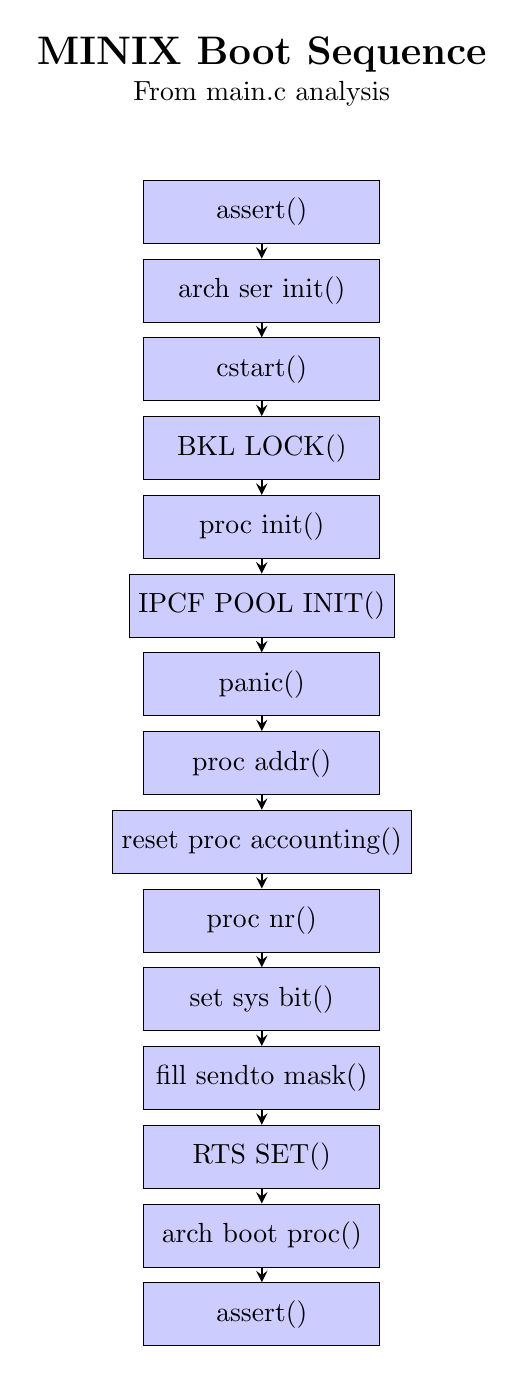
\begin{tikzpicture}[
    box/.style={rectangle, draw=black, fill=blue!20, minimum width=3cm, minimum height=0.8cm},
    arrow/.style={->, >=stealth, thick}
]

% Title
\node[font=\Large\bfseries] at (0, 0) {MINIX Boot Sequence};
\node[font=\normalsize] at (0, -0.5) {From main.c analysis};

\node[box] (stage0) at (0, -2) {assert()};
\node[box] (stage1) at (0, -3) {arch ser init()};
\draw[arrow] (stage0) -- (stage1);
\node[box] (stage2) at (0, -4) {cstart()};
\draw[arrow] (stage1) -- (stage2);
\node[box] (stage3) at (0, -5) {BKL LOCK()};
\draw[arrow] (stage2) -- (stage3);
\node[box] (stage4) at (0, -6) {proc init()};
\draw[arrow] (stage3) -- (stage4);
\node[box] (stage5) at (0, -7) {IPCF POOL INIT()};
\draw[arrow] (stage4) -- (stage5);
\node[box] (stage6) at (0, -8) {panic()};
\draw[arrow] (stage5) -- (stage6);
\node[box] (stage7) at (0, -9) {proc addr()};
\draw[arrow] (stage6) -- (stage7);
\node[box] (stage8) at (0, -10) {reset proc accounting()};
\draw[arrow] (stage7) -- (stage8);
\node[box] (stage9) at (0, -11) {proc nr()};
\draw[arrow] (stage8) -- (stage9);
\node[box] (stage10) at (0, -12) {set sys bit()};
\draw[arrow] (stage9) -- (stage10);
\node[box] (stage11) at (0, -13) {fill sendto mask()};
\draw[arrow] (stage10) -- (stage11);
\node[box] (stage12) at (0, -14) {RTS SET()};
\draw[arrow] (stage11) -- (stage12);
\node[box] (stage13) at (0, -15) {arch boot proc()};
\draw[arrow] (stage12) -- (stage13);
\node[box] (stage14) at (0, -16) {assert()};
\draw[arrow] (stage13) -- (stage14);

\end{tikzpicture}
\end{document}